% LaTeX Workshop：既存の「pLaTeX (Direct) → PDF」レシピでビルド。
% 目次・相互参照が更新されない場合は、もう一度ビルドする。
% 実施範囲：配布テキスト の2-1 CW-NMR（課題1--3、p. 10）。
% Voigt版の資料一覧は ../README.md を参照。
\documentclass[dvipdfmx,a4paper,11pt]{jsarticle}

\usepackage[a4paper,truedimen,margin=25truemm]{geometry}
\usepackage{amsmath,amssymb}
\usepackage{graphicx}
\usepackage{booktabs}
\usepackage{siunitx}
\usepackage[numbib,notlof,notlot,nottoc]{tocbibind}
\usepackage[hidelinks]{hyperref}
\usepackage{pxjahyper}
\usepackage{float}
\usepackage{placeins}

\graphicspath{{figures/}}
\sisetup{separate-uncertainty=true}
\renewcommand{\refname}{参考文献}

\newcommand{\reporttitle}{核磁気共鳴}

\begin{document}

% ===== 表紙 =====
\hypersetup{pageanchor=false}
\begin{titlepage}
  \centering
  \vspace*{25mm}
  {\Large 物理学実験レポート\par}
  \vspace{15mm}
  {\huge\bfseries \reporttitle\par}
  \vspace{25mm}
  \vfill
\end{titlepage}
\hypersetup{pageanchor=true}

\tableofcontents
\clearpage

\section{実験背景・目的}
\label{sec:purpose}

\subsection{実験背景}
核磁気共鳴（nuclear magnetic resonance; NMR）は、静磁場中に置かれた原子核の磁気モーメントが、特定の周波数の高周波磁場に応答する現象である。
磁気モーメントは核スピンの角運動量に比例し、その比例係数である磁気回転比は核種によって異なる。
したがって、共鳴周波数と磁場の関係を利用することで、特定の核種の信号を選択して観測できる\cite{manual}。

共鳴条件だけでなく、核スピン系の緩和も観測信号を決める。
静磁場に平行な磁化が熱平衡値へ戻る過程と、垂直な磁化が減衰する過程は、それぞれスピン-格子緩和時間$T_1$とスピン-スピン緩和時間$T_2$で特徴づけられる。
核磁気共鳴が高周波磁場への共鳴応答を指すのに対し、核磁気緩和は励起された磁化が平衡状態へ向かう過程を指す。
連続的な励起の下での定常的な吸収を理解するには、これらの両方を考える必要がある。

本実験では、硫酸銅水溶液中の水素核を対象に、CW-NMRと呼ばれる、連続的に振動
磁場をかける方法による測定を行った。
静磁場に低周波の変調磁場を重ね、高周波磁場の周波数を掃引することで共鳴信号を検出する。
直接記録する量は周波数とロックインアンプの出力電圧であり、微小変調の条件では、この出力の周波数依存性は共鳴吸収線の微分形に対応する。

%演習では、核スピンの磁気モーメントを古典的なベクトルとして扱い、静磁場中の歳差運動から共鳴条件を考えた。
%静磁場に垂直な高周波磁場の回転成分が歳差運動と同じ向き・同じ角周波数で回ると、その成分は歳差運動とともに回る座標系で時間に依存しない横磁場となる。
%この横磁場が磁化の向きを変える。このときの高周波磁場の角周波数は、ラーモア角周波数$|\gamma|B_0$に等しい。

\subsection{実験目的}
本実験の目的は、CW-NMRによって水素核の共鳴信号を検出し、共鳴条件と信号の検出方法を理解することである。
まず、静磁場を固定して高周波磁場の周波数を掃引し、硫酸銅水溶液の共鳴信号を測定する。
次に、試料位置を変えて共鳴周波数、線幅および信号強度の位置依存性を調べ、永久磁石の磁場分布と、NMR測定に必要な磁場の一様性について検討する。
さらに、試料位置を固定して磁場変調の振幅および周波数を変え、測定条件が共鳴信号に与える影響を調べる。
これにより、観測される線幅に含まれる測定系の影響を検討し、物質固有の横緩和時間$T_2$を評価するための条件を考察する。
% 変調周波数依存性はreadme.mdに記された追加測定。テキストp. 10の課題3は振幅依存性。

\section{実験方法・原理}
\label{sec:methods}

\subsection{測定原理}


\subsubsection{磁気モーメントの歳差運動と共鳴条件}
演習問1--5では磁場を$\boldsymbol{H}$と書く。この記号は、本稿の他の箇所で$\boldsymbol{B}$と表すSI単位系の磁束密度を指す。
演習の$z$軸は静磁場方向に取る。試料位置を表す実験座標$(x,z)$の定義は\ref{sec:method-cw}節で述べる。

\paragraph{演習問1　円運動と磁気回転比}
質量$m$、電荷$q$の粒子が半径$a$の円軌道を角速度$\omega\boldsymbol{e}_z$で回るとする。
速さが$a\omega$であることから、角運動量$\boldsymbol{J}$、電流$I$、磁気モーメント$\boldsymbol{\mu}$は順に
\begin{align}
 \boldsymbol{J}&=\boldsymbol{r}\times\boldsymbol{p}
   =a\,(ma\omega)\boldsymbol{e}_z=ma^2\omega\boldsymbol{e}_z,\\
 I&=\frac{q}{T}=q\left(\frac{2\pi a}{a\omega}\right)^{-1}
   =\frac{q\omega}{2\pi},\\
 \boldsymbol{\mu}&=I\pi a^2\boldsymbol{e}_z
   =\frac{q\omega}{2\pi}\,\pi a^2\boldsymbol{e}_z
   =\frac{qa^2\omega}{2}\boldsymbol{e}_z
\end{align}
となる。ここで$T$は一周の周期である。$\boldsymbol{\mu}=\gamma\boldsymbol{J}$より、この古典模型では
\begin{equation}
 \gamma=\frac{qa^2\omega}{2}\frac{1}{ma^2\omega}=\frac{q}{2m}
\end{equation}
を得る。
以下の運動方程式では、$\gamma$に対象とする核種の磁気回転比を用いる。

\paragraph{演習問2　静磁場中の歳差運動}
磁気モーメントに働くトルクは$\mathrm{d}\boldsymbol{J}/\mathrm{d}t
=\boldsymbol{\mu}\times\boldsymbol{H}$である。$\boldsymbol{\mu}=\gamma\boldsymbol{J}$から、
静磁場$\boldsymbol{H}=(0,0,H_0)$のもとでの運動方程式は
\begin{equation}
  \frac{\mathrm{d}\boldsymbol{\mu}}{\mathrm{d}t}
   =\gamma
   \begin{pmatrix}\mu_x\\\mu_y\\\mu_z\end{pmatrix}
   \times\begin{pmatrix}0\\0\\H_0\end{pmatrix}
   =\gamma H_0\begin{pmatrix}\mu_y\\-\mu_x\\0\end{pmatrix}
\end{equation}
となる。$\dot{\mu}_x=\gamma H_0\mu_y$をさらに微分し、$\dot{\mu}_y=-\gamma H_0\mu_x$を代入すると、
$\ddot{\mu}_x=\gamma H_0\dot{\mu}_y=-(\gamma H_0)^2\mu_x$となる。
これを解き、$\mu_y=\dot{\mu}_x/(\gamma H_0)$と$\dot{\mu}_z=0$を用いると
\begin{equation}
  \boldsymbol{\mu}=
  \begin{pmatrix}
   A\cos(\gamma H_0 t+\phi)\\
   -A\sin(\gamma H_0 t+\phi)\\
   \mu_{z0}
  \end{pmatrix}
\end{equation}
を得る。$A$、$\phi$、$\mu_{z0}$は初期条件で決まる。磁気モーメントは$z$軸となす角を保ち、角周波数$|\gamma H_0|$で歳差運動する。回転の向きを含めた角速度は$-\gamma H_0$である。

\paragraph{演習問3　回転座標系での運動}
$z$軸の周りを回る座標系を取り、ここからは$\omega$を回転の向きを含む角速度とする。
横方向の基底を$\boldsymbol{i}$、$\boldsymbol{j}$とする。
基底は$\dot{\boldsymbol{i}}=\omega\boldsymbol{e}_z\times\boldsymbol{i}$、
$\dot{\boldsymbol{j}}=\omega\boldsymbol{e}_z\times\boldsymbol{j}$を満たす。
$\boldsymbol{\mu}=\mu_{rx}\boldsymbol{i}+\mu_{ry}\boldsymbol{j}+\mu_{rz}\boldsymbol{e}_z$を実験室座標系で微分すると
\begin{align}
 \frac{\mathrm{d}\boldsymbol{\mu}}{\mathrm{d}t}
 &=\dot{\mu}_{rx}\boldsymbol{i}+\dot{\mu}_{ry}\boldsymbol{j}
   +\dot{\mu}_{rz}\boldsymbol{e}_z
   +\mu_{rx}\dot{\boldsymbol{i}}+\mu_{ry}\dot{\boldsymbol{j}}\\
 &=\frac{\delta\boldsymbol{\mu}_r}{\delta t}
   +\omega\boldsymbol{e}_z\times\boldsymbol{\mu}.
\end{align}
ここで$\delta\boldsymbol{\mu}_r/\delta t$は回転座標系での成分の時間微分である。
実験室座標系の運動方程式$\mathrm{d}\boldsymbol{\mu}/\mathrm{d}t
=\gamma\boldsymbol{\mu}\times\boldsymbol{H}$を代入すると、
\begin{align}
 \frac{\delta\boldsymbol{\mu}_r}{\delta t}
 &=\gamma\boldsymbol{\mu}\times\boldsymbol{H}
   -\omega\boldsymbol{e}_z\times\boldsymbol{\mu}\\
 &=\gamma\boldsymbol{\mu}\times
    \left(\boldsymbol{H}+\frac{\omega}{\gamma}\boldsymbol{e}_z\right)
\end{align}
を得る。高周波磁場$2H_1\cos(\omega t)\boldsymbol{e}_x$は振幅$H_1$の二つの回転成分に分解できる。
歳差運動と同じ向きに回る成分に座標系を合わせると、この成分は$H_1\boldsymbol{i}$となる。
逆向きの成分は角周波数$2|\omega|$で回るため、共鳴近傍ではその寄与を無視する。有効磁場は
\begin{equation}
 \boldsymbol{H}_{\mathrm{eff}}
 =\left(H_0+\frac{\omega}{\gamma}\right)\boldsymbol{e}_z
   +H_1\boldsymbol{i}
\end{equation}
となる。$\omega=-\gamma H_0$で縦成分が消え、磁気モーメントは回転座標系の$\boldsymbol{i}$軸の周りを歳差運動する。
共鳴周波数は
\begin{equation}
  f_0=\frac{|\gamma H_0|}{2\pi}
  \label{eq:resonance}
\end{equation}
となる。

\subsubsection{ブロッホ方程式と共鳴吸収線}
多数の核スピンの磁気モーメントを単位体積あたりで足し合わせた量を磁化$\boldsymbol{M}$とする。
緩和を現象論的に取り入れると、その時間変化はブロッホ方程式
\begin{equation}
 \frac{\mathrm{d}\boldsymbol{M}}{\mathrm{d}t}
 =\gamma\boldsymbol{M}\times\boldsymbol{H}
 -\frac{M_x\boldsymbol{e}_x+M_y\boldsymbol{e}_y}{T_2}
 -\frac{M_z-M_0}{T_1}\boldsymbol{e}_z
\end{equation}
で表される。$M_0$は静磁場方向の熱平衡磁化である。
$T_1$は縦磁化の回復、$T_2$は横磁化の減衰を特徴づける時間である。
高周波磁場によって供給されたエネルギーが周囲の自由度へ移ることで、連続的な励起の下でも定常的な吸収が可能になる。

\paragraph{演習問4　定常磁化の円軌跡}
回転座標系の磁化を$(M_i,M_j,M_z)$とする。試料に静磁場および回転磁場をかけているとき
\begin{align}
  \frac{\mathrm{d} M_z}{\mathrm{d} t}= -\gamma M_j H_1 + \frac{M_0-M_z}{T_1},\\
  \frac{\mathrm{d} M_i}{\mathrm{d} t}= \gamma M_j\left(H_0+\frac{\omega}{\gamma}\right) - \frac{M_i}{T_2},\\
  \frac{\mathrm{d} M_j}{\mathrm{d} t}= \gamma \left[M_z H_1 -M_i\left(H_0+\frac{\omega}{\gamma}\right) \right]- \frac{M_j}{T_2}
\end{align}


$\omega_0=\gamma H_0$、$c=\omega_0+\omega$とおくと、
定常状態ではブロッホ方程式の各成分の時間微分がゼロになるので、
\begin{equation}
 0=cM_j-\frac{M_i}{T_2},\qquad
 0=\gamma H_1 M_z-cM_i-\frac{M_j}{T_2},\qquad
 0=-\gamma H_1 M_j+\frac{M_0-M_z}{T_1}
\end{equation}
を得る。高周波磁場が十分弱く$\gamma^2 H_1^2T_1T_2\ll 1$なら$M_z\simeq M_0$となり、横成分は
\begin{equation}
 M_i=\frac{\gamma cH_1T_2^2}{1+T_2^2c^2}M_0,\qquad
 M_j=\frac{\gamma H_1T_2}{1+T_2^2c^2}M_0
\end{equation}
となる。両成分の二乗を足すと
\begin{align}
 M_i^2+M_j^2
 &=\frac{\gamma^2 H_1^2T_2^2M_0^2}{(1+T_2^2c^2)^2}
   (T_2^2c^2+1)\\
 &=\frac{\gamma^2 H_1^2T_2^2M_0^2}{1+T_2^2c^2}
   =(\gamma H_1T_2M_0)M_j.
\end{align}
$A=\gamma H_1T_2M_0$と置くと、$M_i^2+M_j^2-AM_j=0$である。平方完成すると
\begin{equation}
 M_i^2+\left(M_j-\frac{A}{2}\right)^2=\left(\frac{A}{2}\right)^2
\end{equation}
を得る。したがって、周波数を変えたときの定常横磁化の先端は、回転座標系の$(M_i,M_j)$平面で
中心$(0,A/2)$、半径$A/2$の円上をたどる。
周波数を固定したときは回転座標系の成分が一定となり、実験室座標系では磁化が$z$軸の周りを一定の傾きで回転する。

\paragraph{演習問5　周期平均の吸収電力}
実験室座標系の磁場は$\boldsymbol{H}=H_0\boldsymbol{e}_z+2H_1\cos(\omega t)\boldsymbol{e}_x$である。
$M_x=M_i\cos(\omega t)-M_j\sin(\omega t)$であり、$M_z$は一定なので、
\begin{equation}
 \boldsymbol{H}\cdot\frac{\mathrm{d}\boldsymbol{M}}{\mathrm{d}t}
 =-2\omega H_1\bigl[M_i\sin(\omega t)\cos(\omega t)
                    +M_j\cos^2(\omega t)\bigr]
\end{equation}
となる。一周期$\tau=2\pi/|\omega|$での$\sin(\omega t)\cos(\omega t)$の平均は$0$であり、
$\cos^2(\omega t)=\{1+\cos(2\omega t)\}/2$の平均は$1/2$である。
したがって、単位体積あたりの周期平均の吸収電力$P$は
\begin{align}
 P &= \frac{1}{\tau}\int_0^\tau
      \boldsymbol{H}\cdot\frac{\mathrm{d}\boldsymbol{M}}{\mathrm{d}t}\,\mathrm{d}t
    =-2\omega H_1 M_j\,\frac{1}{2}\\
   &= -\omega H_1 M_j
    = -\frac{\gamma\omega H_1^2T_2M_0}{1+T_2^2(\omega_0+\omega)^2}.
\end{align}
水素核では$\gamma>0$で、歳差運動と同じ向きに回る成分には$\omega<0$を取るため、$P$は正になる。
同位相の成分$M_i$は分散に、位相が$90^\circ$ずれた成分$M_j$は吸収に対応し、周期平均の電力には$M_j$が寄与する。
$f=|\omega|/(2\pi)$とおくと$\omega_0+\omega=2\pi(f_0-f)$となる。共鳴近傍で分子の$\omega$の変化を無視すると、吸収線形$L(f)$は
\begin{equation}
 L(f)\propto\frac{1}{1+\{2\pi(f-f_0)T_2\}^2}
\label{eq:bloch-lorentz}
\end{equation}
というローレンツ型で表される。この理想的な吸収線の半値全幅は
$\Delta f_{\mathrm{FWHM}}=1/(\pi T_2)$である。

\subsubsection{磁場変調とロックイン検出}
静磁場と同じ方向に低周波の変調磁場を加えると、試料位置での磁場は
\begin{equation}
 \boldsymbol{B}(t)=\{B_0+\Delta B\cos(2\pi f_m t)\}\boldsymbol{e}_z
 +B_{\mathrm{RF}}\cos(2\pi f t)\boldsymbol{e}_x
\end{equation}
と表される。$f_m$と$\Delta B$は変調磁場の周波数と振幅、$f$は掃引する高周波磁場の周波数である。
このとき、共鳴周波数は振幅$\Delta f_m=|\gamma|\Delta B/(2\pi)$で変動する。
共鳴吸収を発振器の電圧変化として検出し、そのうち変調周波数$f_m$に同期する成分をロックインアンプで取り出す。

変調に対して応答を準静的に扱うことができ、かつ$\Delta f_m$が吸収線幅に対して十分小さい場合、吸収信号の変化は一次の展開によって
\begin{equation}
 L\!\left(f-\Delta f_m\cos(2\pi f_m t)\right)
 \simeq L(f)-\Delta f_m\frac{\mathrm{d}L(f)}{\mathrm{d}f}\cos(2\pi f_m t)
\end{equation}
と表される。したがって、符号を含むロックインの同相出力は、吸収線の周波数微分に比例する。
%出力の符号と大きさは参照位相と測定系の利得にも依存する。
%変調幅が大きい場合や応答の遅れが無視できない場合には、この微分近似だけでは波形を表せない。

\subsection{実験装置}
CW-NMR装置は、永久磁石、試料コイルを含むLC発振回路、周波数可変用電源、周波数カウンタ、磁場変調コイル、ロックインアンプ、デジタル電圧計およびPCから構成される\cite{manual}。
硫酸銅水溶液を入れたテフロン製容器には試料コイルが巻かれており、同軸ケーブルを介してコンデンサに接続され、LC回路を構成する。
試料コイルは永久磁石の磁極間に配置される。

周波数可変用電源の出力電圧によって発振周波数を変え、周波数カウンタでその値を測定する。
水素核の共鳴吸収に伴う発振器の電圧変化をロックインアンプへ入力し、磁場変調に同期した成分を検出する。
ロックインアンプの出力はデジタル電圧計で読み取り、周波数の測定値とともにPCへ取り込む。

\subsection{CW-NMRの測定手順・条件}
\label{sec:method-cw}
\subsubsection{水素核の共鳴検出（課題1）}
永久磁石の磁場と試料位置を固定し、発振周波数を掃引して水素核の共鳴信号を測定した。
この測定での試料位置の座標は不明である。
テキストに示された磁場の目安$B_0\simeq\SI{0.38}{\tesla}$と、水素核の周波数・磁場比
$|\gamma|/(2\pi)=\SI{42.5759}{\mega\hertz\per\tesla}$を用いると、共鳴周波数は約\SI{16.2}{\mega\hertz}と予想される。

発振周波数を変えながら周波数カウンタの値とロックイン出力を記録し、共鳴に対応する出力の変化を測定した。
課題1・2のテキスト指定値は、変調周波数\SI{280}{\hertz}、変調電圧\SI{1.3}{\volt}、ロックインアンプの感度（Sensitivity）\SI{100}{\milli\volt}、時定数（Time Constant）\SI{1}{\second}である\cite{manual}。
実際の測定では、ロックインアンプの時定数を\SI{200}{\milli\second}とし、課題1・2の各測定点での待ち時間（Delay Time）を\SI{0.5}{\second}とした。
課題1の記録では、発振周波数は約\SI{15.983}{\mega\hertz}から\SI{16.154}{\mega\hertz}まで上昇した。課題2の解析に用いた波形も上り掃引であった。
%制御電圧の掃引設定、変調電圧の表示値が実効値・片振幅・両振幅のいずれかは確認できなかった。

\subsubsection{磁場・線幅・信号強度の位置依存性（課題2）}
静磁場に垂直な平面内に実験座標$(x,z)$を取り、両軸の単位を\si{\centi\metre}とした。$x$の正方向は装置の奥側、$z$の正方向は鉛直上向きである。
装置の中央での座標読みは$(4.5,4.5)$であり、各軸について中央から$\pm\SI{2}{\centi\metre}$の範囲を基本として試料を動かした。
各位置で周波数掃引を行って共鳴信号を測定し、座標読みをデータファイル名に記録した。
各位置の共鳴周波数を比較することで磁場分布を調べ、あわせて共鳴線幅と信号強度の位置依存性を検討する。
配布テキストは両方向に\SI{0.5}{\centi\metre}刻みで中央からおよそ$\pm\SI{2}{\centi\metre}$の測定を指定している\cite{manual}。

%11月4日の$(6.0,4.0)$では周波数刻みを細かくして再測定した。11月10日の待ち時間を変えた試行4件は、通常測定の集計から除いた。

\subsubsection{磁場変調振幅・周波数依存性（課題3および追加測定）}
課題3では、課題2で求めた最大磁場の位置に試料を置くことが指定されていた\cite{manual}。
しかし、今回の位置依存測定からは最大磁場の位置を特定できなかったため、11月4日の変調条件の測定では、試料を装置の中央$(x,z)=(4.5,4.5)$に固定した。
以下の結果は、中央位置における変調条件への依存性を示す。
変調周波数を\SI{280}{\hertz}に固定する系列では、変調コイルの駆動電圧の表示値を
0.5、1.0、1.3、1.5、2.0、2.5、3.0、3.5、4.0、4.5\,Vの10通りとした。
追加測定では、駆動電圧の表示値を\SI{1.3}{\volt}に固定し、変調周波数を\SIrange{20}{400}{\hertz}の範囲で\SI{20}{\hertz}刻みの20通りとした。
両系列に共通する設定は\SI{1.3}{\volt}・\SI{280}{\hertz}である。
各設定で高周波磁場の周波数を低い側から掃引し、共鳴信号を記録した。測定プログラムの待ち時間（Delay Time）は\SI{1}{\second}とした。
ロックインアンプの時定数は\SI{200}{\milli\second}とした。


\subsection{LabVIEWによる測定制御・データ取得}
LabVIEWで測定を制御し、データを取得した。測定用VIは、試作版の \texttt{takeuchi\_2014\_01.vi} および \texttt{takeuchi\_2026\_01.vi} と同等のものである。
測定用VIでは、周波数可変用電源を制御し、周波数カウンタとデジタル電圧計の測定値を取得して保存した。
周波数軸には周波数カウンタの実測値を用いる。
保存された周波数と信号の組から共鳴周波数、線幅、信号強度を求める処理は、測定後にPythonで行った。

\subsection{Pythonによるデータ解析}
\label{sec:data-analysis}
各データファイルの第1列を周波数（Hz）、第2列をロックイン出力の記録値として読み込んだ。
信号の値は保存された数値の単位で扱い、フィットには平滑化していない測定点を用いた。

\paragraph{Voigt吸収線と磁場変調の基本波}
個々の場所の吸収線をローレンツ型とし、試料内の共鳴周波数が標準偏差$\sigma_f$のガウス分布に従うと仮定した。
両者の畳み込みであるVoigt吸収線を$V(u;\Gamma,\sigma_f)$とする。ここで$u=f-f_0$は共鳴中心からの周波数差、$\Gamma$はローレンツ成分の半値半幅である。
具体的には、面積を1に規格化したローレンツ吸収線$\ell$と、局所的な共鳴周波数のずれ$\delta$の分布$G$を
\begin{equation}
 \ell(u;\Gamma)=\frac{\Gamma}{\pi(u^2+\Gamma^2)},\qquad
 G(\delta;\sigma_f)=\frac{1}{\sqrt{2\pi}\sigma_f}
 \exp\!\left(-\frac{\delta^2}{2\sigma_f^2}\right)
\end{equation}
とし、吸収線を
\begin{align}
 V(u;\Gamma,\sigma_f)
 &=\int_{-\infty}^{\infty}G(\delta;\sigma_f)\ell(u-\delta;\Gamma)\,\mathrm{d}\delta\notag\\
 &=\frac{\Gamma}{\pi\sqrt{2\pi}\sigma_f}
 \int_{-\infty}^{\infty}
 \frac{\exp\{-\delta^2/(2\sigma_f^2)\}}{(u-\delta)^2+\Gamma^2}\,\mathrm{d}\delta
 \label{eq:voigt-convolution}
\end{align}
で表した。これは、中心が$\delta$だけずれた吸収線を、その存在割合$G(\delta;\sigma_f)\,\mathrm{d}\delta$で重み付けして足し合わせる操作である。
$\sigma_f$は共鳴周波数の分布幅であり、推定値の不確かさとは異なる。$\sigma_f=0$では分布が一点に集中する極限を取り、$V=\ell$とする。

磁場変調による共鳴周波数の片振幅を$a$とし、磁化が変調に準静的に追従すると仮定して、基本波成分を
\begin{equation}
 S(u;\Gamma,\sigma_f,a)=
 \frac{1}{\pi a}\int_0^{2\pi}
 V(u+a\cos\theta;\Gamma,\sigma_f)\cos\theta\,\mathrm{d}\theta
 \qquad (a>0)
 \label{eq:finite-modulation}
\end{equation}
とした。$\theta$は変調の位相であり、$\cos\theta$を掛けて一周期積分することで変調に同期する成分を取り出す。
$a$で割った倍率と信号の符号は、自由係数$A$に含めた。$a=0$では、この式の極限であるVoigt吸収線の微分
\begin{equation}
 S(u;\Gamma,\sigma_f,0)=\frac{\mathrm{d}V(u;\Gamma,\sigma_f)}{\mathrm{d}u}
 =-\frac{2\Gamma}{\pi}\int_{-\infty}^{\infty}
 G(\delta;\sigma_f)\frac{u-\delta}{\{(u-\delta)^2+\Gamma^2\}^2}\,\mathrm{d}\delta
 \label{eq:voigt-derivative}
\end{equation}
を用いた。この$a=0$は正規化した波形の微小変調極限を意味し、実験で変調磁場を加えなかったことを意味しない。
最終的な予測信号を
\begin{equation}
 \hat y(f)=A S(f-f_0;\Gamma,\sigma_f,a)+b_0+b_1(f-f_{\mathrm{ref}})
 \label{eq:task1-fit}
\end{equation}
とし、$f_0,\Gamma,\sigma_f,a,A,b_0,b_1$を全測定点に対する非加重最小二乗法で推定した。
$f_{\mathrm{ref}}$は固定した計算上の基準周波数で、$b_0$と$b_1$は直線背景の切片と傾きである。
この計算には\texttt{nmr\_joint\_noise.py}を用いた。

\paragraph{課題2・3への適用とモデルの比較}
課題2では全座標で式\eqref{eq:voigt-derivative}を用い、課題3では式\eqref{eq:finite-modulation}の変調片振幅$a$を条件ごとに推定した。
いずれも式\eqref{eq:task1-fit}の直線背景を加えた。両課題について、微分ローレンツ型、微分Voigt型、有限変調ローレンツ型、有限変調Voigt型の4種類を同じ測定点で比較した。
基準となる微分ローレンツ型の中心から前後\SI{6}{\kilo\hertz}を幅\SI{2}{\kilo\hertz}の区間に分け、一つずつフィットから外した。
残りの点で再推定した波形と、外した全点の測定値との差の二乗平均平方根（予測RMS）を求めた。これは同じ掃引内の未使用区間に対する予測を評価する量である。

\paragraph{線幅・信号強度・磁場の定義}
吸収線の半値全幅は変調前の$V(u)$について、$V(u)=V(0)/2$を満たす二点の間隔とした。
観測波形の山谷間隔は背景を引いた基本波の極大・極小の周波数差、信号強度は同じ二点の出力差とした。
磁束密度は式\eqref{eq:resonance}により、$|\gamma|/(2\pi)=\SI{42.5759}{\mega\hertz\per\tesla}$を用いて共鳴中心から換算した。

\subsection{不確かさの評価方法}
\label{sec:analysis-uncertainty}
1掃引から求めた共鳴周波数と線幅のばらつきを評価した。測定順に$i=1,\ldots,n$とし、周波数$f_i$でのフィット値を$\hat y_i$、模擬測定値を$y_i^*$とする。

\paragraph{課題1：独立な加法雑音と相関する振幅揺らぎ}
1250点の残差で選んだ次のモデルから模擬波形を生成した（パラメトリック・ブートストラップ\cite{efron_bootstrap}）。
\begin{align}
 y_i^* &= \hat y_i + s_i Z_i + c\,h_i G_i, \label{eq:noise-task1}\\
 G_i &= \rho G_{i-1}+\sqrt{1-\rho^2}\,W_i \qquad (i\geq 2).
\end{align}
$Z_i$、$W_i$、初期値$G_1$は互いに独立な標準正規乱数とした。第1の雑音項$s_i Z_i$は点ごとに独立で、
その標準偏差$s_i$の対数は周波数の一次関数として残差から推定した。
第2の雑音項では、背景を引いたフィット信号$h_i$に相対振幅の揺らぎ$cG_i$を掛けた。
推定値は$c=0.0831$、$\rho=0.799$であり、隣り合う点の振幅揺らぎは前の点の変動を一部引き継ぐ。
元の推定曲線は変調片振幅$a=0$であったが、模擬波形の再フィットでは$a>0$の解も許した。

\paragraph{課題2・3：残差のブロックごとの符号反転}
課題2・3は1掃引あたり67～300点で、位置や変調条件によって信号の強さや背景が異なる。課題1で選んだ雑音モデルが各条件にも適合するかは未検証である。
そこで各掃引の実測残差$r_i=y_i-\hat y_i$とその平均$\bar r$を用い、近接点の残差に共通の重みを掛けるブロック・ワイルド・ブートストラップ\cite{smeekes_wilms_bwb}を適用した。
\begin{equation}
 y_i^*=\hat y_i+\sqrt{\frac{n}{n-p}}\,(r_i-\bar r)\,\xi_{b(i)},
 \qquad \Pr(\xi_b=+1)=\Pr(\xi_b=-1)=\tfrac12 .
 \label{eq:noise-block}
\end{equation}
$n$は1掃引の測定点数、$p$はその掃引で推定するパラメータ数（課題2で6、課題3で7）である。
残差の標本平均$\bar r=n^{-1}\sum_i r_i$を引いて残差を中心化した。今回は背景の切片を含む非加重最小二乗フィットのため、$\bar r$は数値誤差の範囲でゼロになる。
フィットに伴って残差のばらつきが小さくなる分を補うため、分散の分母を$n$から$n-p$に換算する係数の平方根$\sqrt{n/(n-p)}$を各残差に掛けた。これは線形回帰で用いるHC1型の自由度補正\cite{mackinnon_hc1}を、相関のある非線形フィットに近似的に適用したものである。
測定順に$\lceil n^{1/3}\rceil$点（5～7点）ずつに区切り、試行ごとに開始位置を無作為にずらした。点$i$を含むブロック$b(i)$ごとに符号を独立に選び、補正した残差を元の周波数で元のフィット曲線$\hat y_i$に加えた。

\paragraph{模擬回数と標準不確かさ}
課題1は300回、課題2・3は各波形につき120回再フィットし、各量の再推定値の標本標準偏差を標準不確かさとした。
回数は計算上の設定である。1回の掃引から得る推定値のばらつきを求めているため、試行回数の平方根では割らない。
課題1の共鳴周波数では、最初の100回、200回、全300回で標準偏差はそれぞれ21.3、20.7、\SI{21.4}{\hertz}であった。
課題1の共鳴周波数の標準不確かさは、信号雑音による再推定値のばらつきから約21 Hzと求めた。
周波数の保存刻みは10 Hzであり、各点に独立な丸め誤差を仮定した感度確認では、共鳴周波数のばらつきは約0.7 Hzであった。
周波数カウンタの校正に由来する不確かさは未評価である。

\section{結果}
\label{sec:results}

\subsection{水素核の共鳴信号（課題1）}
10月20日の上り掃引（\texttt{20261020\_KITtest01.dat}）の1250点を解析した。
図\ref{fig:task1-fit}に共鳴付近の測定値、フィット曲線、残差を示す。
測定信号は低周波数側に山、高周波数側に谷を持ち、共鳴付近で符号が反転した。
有限変調Voigtモデルで残差平方和が最小となった解は、微小変調極限のVoigt微分形であった。
微分Voigt型と有限変調Voigt型で共鳴周波数の差は\SI{0.01}{\hertz}未満であり、未使用区間の予測RMSは微分Voigt型の方が小さかった（それぞれ0.090、0.098）。そこで課題1では微分Voigt型を採用した。
この解から求めた共鳴周波数と二種類の幅を表\ref{tab:task1-results}に示す。

\begin{table}[htbp]
  \centering
  \caption{課題1のフィット結果。標準不確かさは、300組の模擬測定から得た再推定値の標本標準偏差である。}
  \label{tab:task1-results}
  \begin{tabular}{lrr}
    \toprule
    量 & 推定値 & 標準不確かさ\\
    \midrule
    共鳴周波数 $f_0$（MHz） & 16.010623 & 0.000021\\
    観測波形の山谷間隔（kHz） & 2.374 & 0.096\\
    変調前のVoigt吸収線の半値全幅（kHz） & 2.99 & 0.35\\
    \bottomrule
  \end{tabular}
\end{table}

\begin{figure}[htbp]
  \centering
  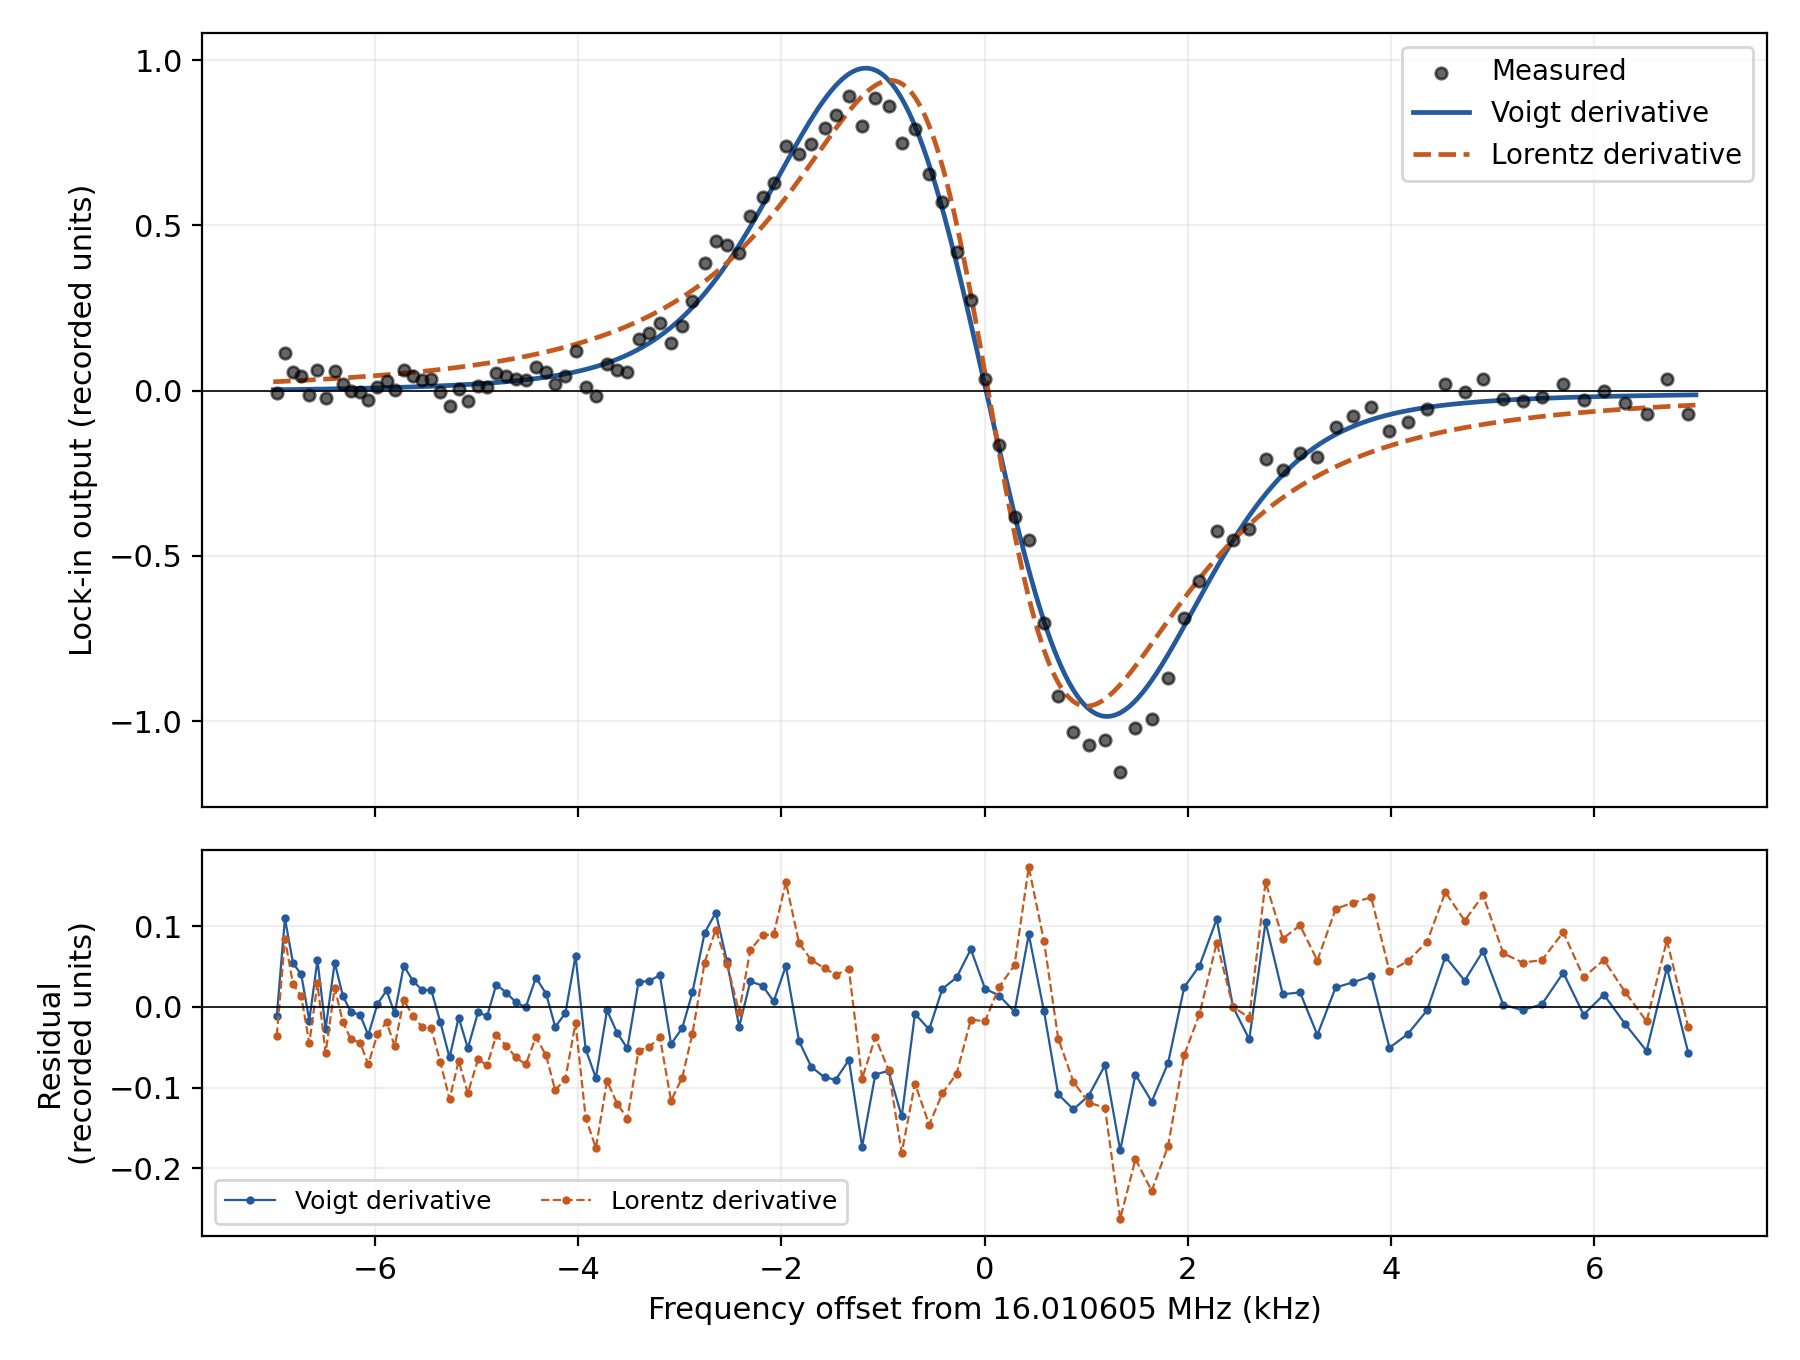
\includegraphics[width=0.86\linewidth]{fig1.png}
  \caption{課題1の共鳴付近の波形と残差。横軸は基準周波数\SI{16.010605}{\mega\hertz}からの差である。
  上段は測定値、Voigt微分型（実線）および微分ローレンツ型（破線）のフィット、下段は各曲線に対する通常の残差（測定値からフィット値を引いた差）である。
  両モデルとも同じ全1250点と直線背景を用いた非加重最小二乗フィットであり、図には共鳴付近を拡大して示す。}
  \label{fig:task1-fit}
\end{figure}

\FloatBarrier



残差の二乗平均平方根は全1250点で0.0507、基準周波数の前後\SI{5}{\kilo\hertz}の75点で0.0647であった。
共鳴付近に限って同じ範囲を比較すると、微分ローレンツ型の値は0.1017であった。
Voigtモデルでも共鳴付近に同符号の残差が続く箇所があり、隣接相関は0.57であった。

\subsection{位置依存性と磁場分布（課題2）}
同一座標では新しい測定を採用した。得られた83座標のうち、基本範囲外の2座標（$x=7$、$z=7$、$z=2.0$のいずれかに該当）と、
共鳴が不明瞭か、フィット範囲や背景の取り方に強く依存した3座標を除外した。残る78座標の推定値を図\ref{fig:task2-position}に示す。
共鳴周波数は式\eqref{eq:resonance}で磁束密度に換算した。色付きの点の換算値は約\SI{375.96}{\milli\tesla}から\SI{376.40}{\milli\tesla}の範囲にある。
$z=4.0$と$z=4.5$の間で磁束密度が大きく変わって見えるが、この付近では測定日も切り替わる。

\begin{figure}[tbp]
  \centering
  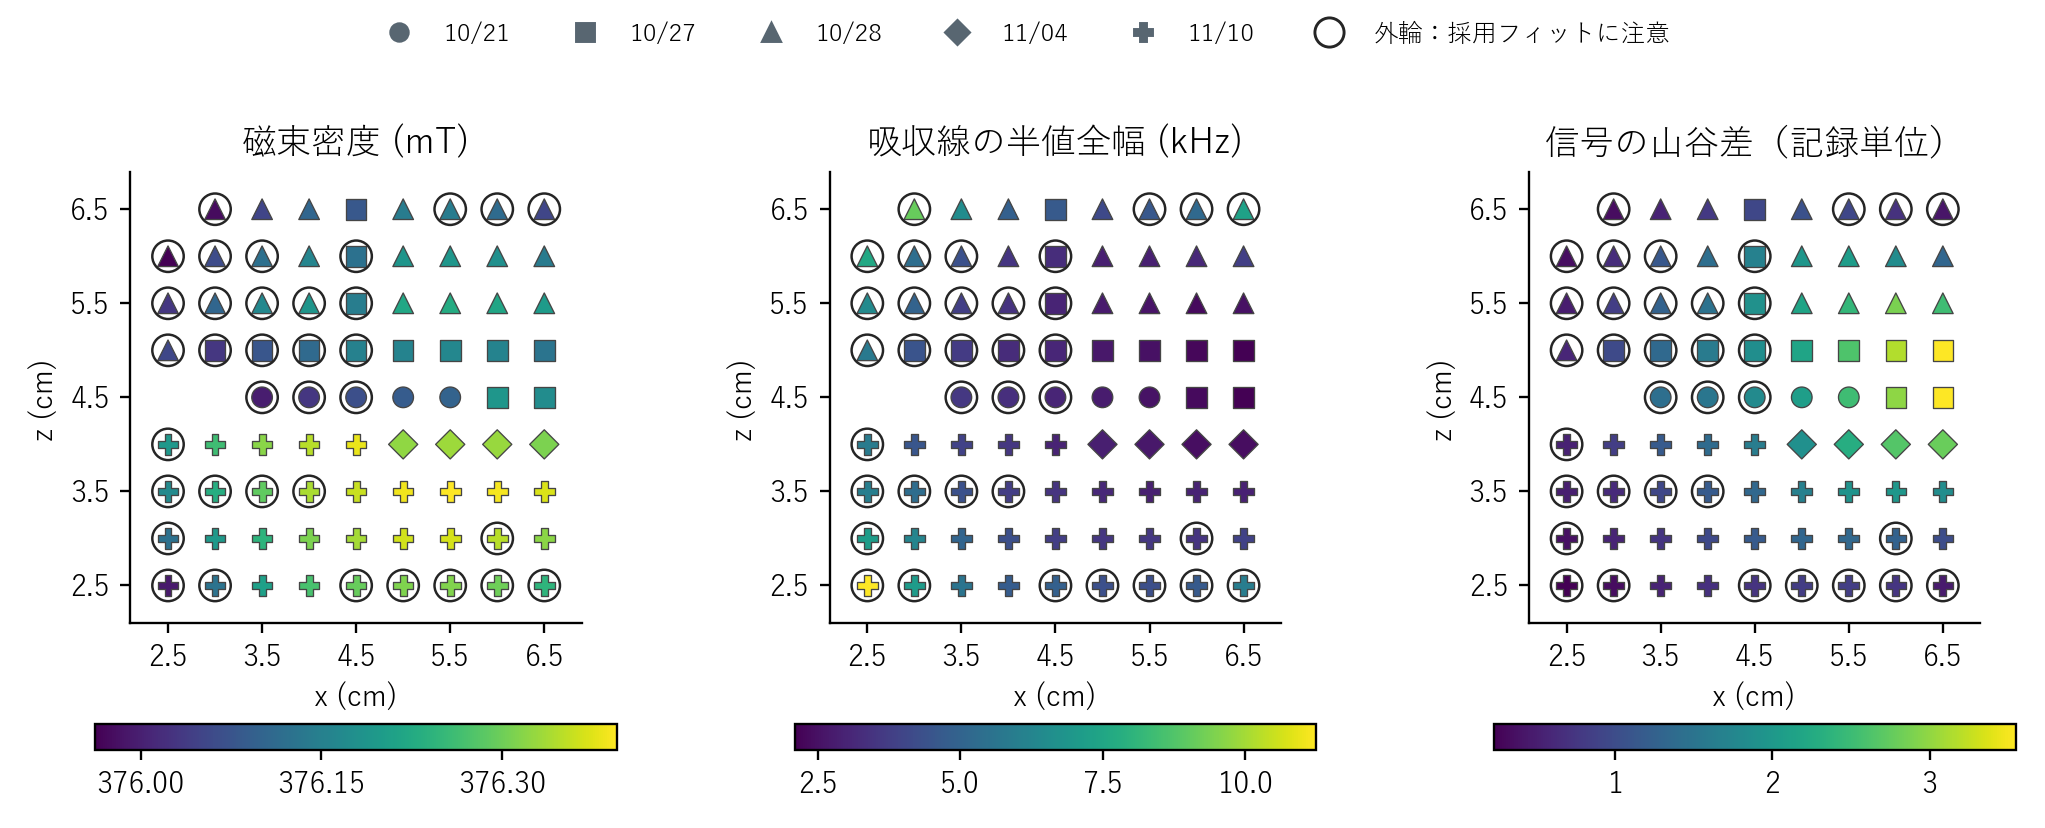
\includegraphics[width=\linewidth]{fig2.png}
  \caption{磁束密度、吸収線の半値全幅、信号強度の位置依存性。色付きの点はフィットの推定値で、形は測定日、点を囲む外輪は微分Voigt型の注意が付いた座標を示す。
  $x$、$z$は装置の座標読み（単位は\si{\centi\metre}）。信号強度は背景を除いたフィット波形の山谷差を記録値の単位で示した。
  磁束密度の換算には測定日間の補正を加えていない。}
  \label{fig:task2-position}
\end{figure}

11月10日の測定内で$x=4.5$を固定して比べると、$z=2.5$から$4.0$にかけて、
磁束密度は\SI{376.295}{\milli\tesla}から\SI{376.381}{\milli\tesla}に増加し、
半値全幅は\SI{4.87}{\kilo\hertz}から\SI{2.97}{\kilo\hertz}に減少した。
同じ区間で、信号の山谷差は0.73から1.62に増加した。

78座標中64座標で、微分Voigt型の予測RMSは微分ローレンツ型より小さく、減少率の中央値は19.9\%であった。
中心の移動量の絶対値の中央値は\SI{27}{\hertz}である一方、推定した吸収線の半値全幅は中央値で12.9\%小さくなった。
有限変調Voigt型で変調片振幅を自由にしても、微分Voigt型より予測RMSが下がったのは78座標中26座標にとどまったため、磁場分布には全座標で微分Voigt型を採用した。
両モデル間の推定値の差の絶対値は、中央値で共鳴周波数が\SI{8.5}{\hertz}、吸収線の半値全幅が\SI{1.10}{\kilo\hertz}であった。したがって、図示した線幅は微分Voigt型による有効線幅として解釈する。

\begin{figure}[htbp]
  \centering
  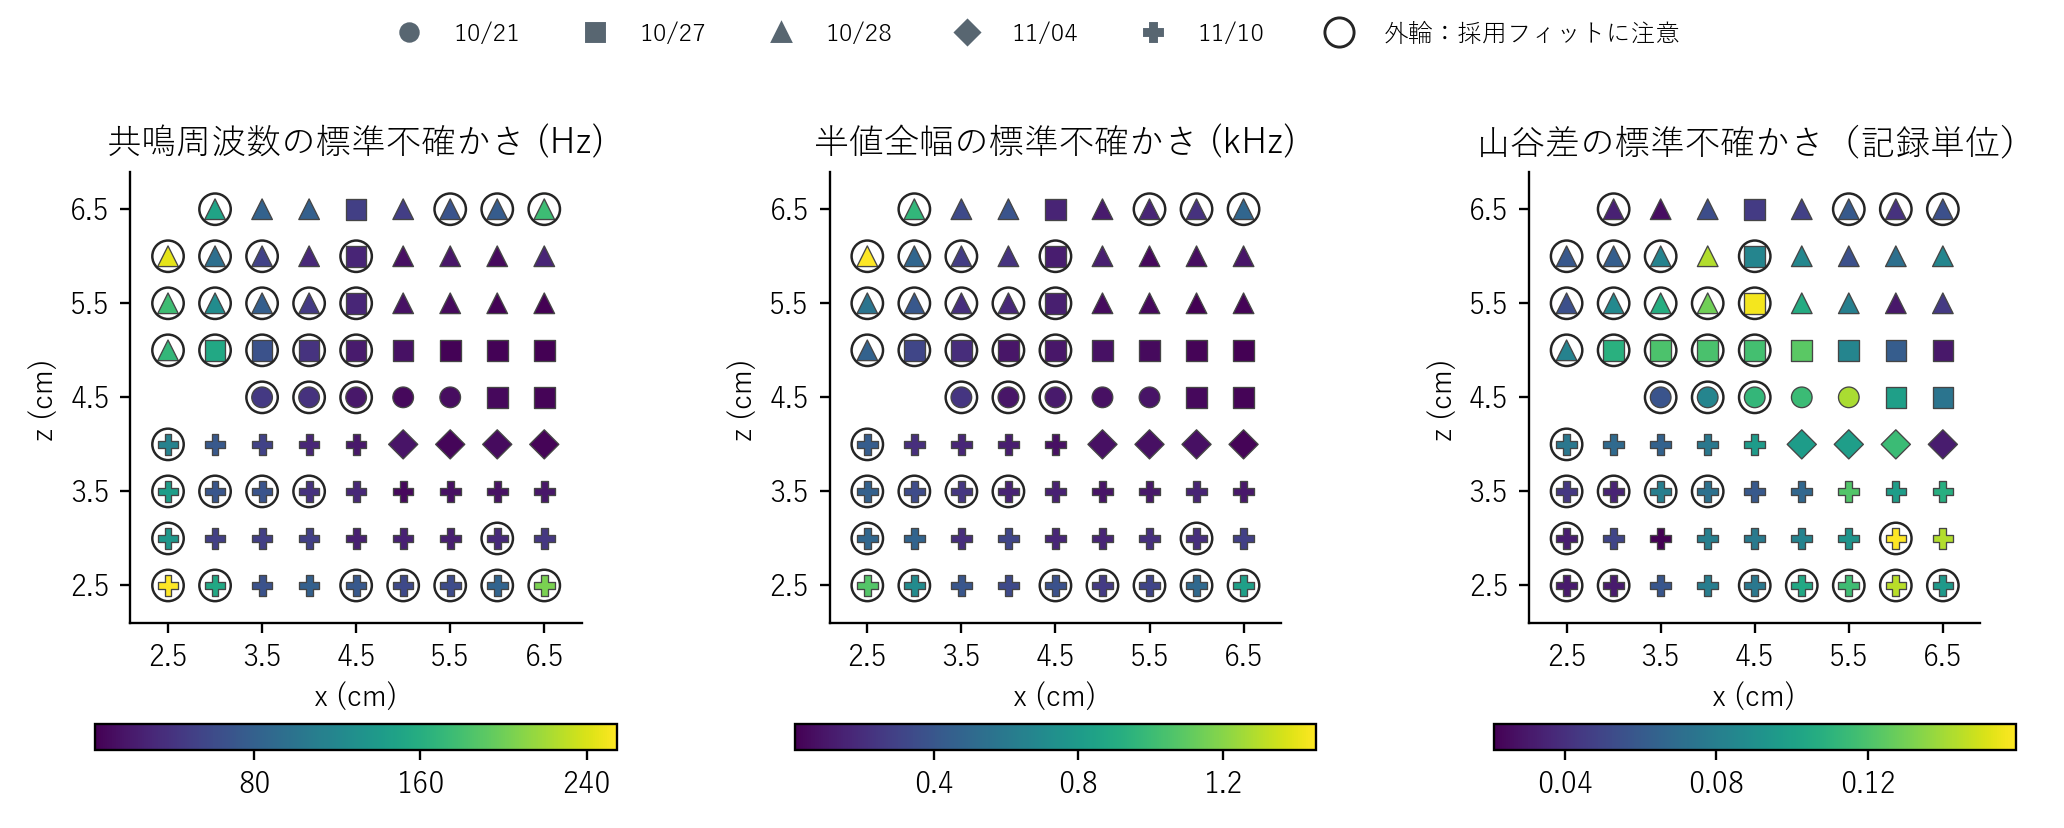
\includegraphics[width=1\linewidth]{fig3.png}
  \caption{78座標の標準不確かさ。外輪は微分Voigt型の注意が付いた座標。共鳴周波数、変調前の吸収線の半値全幅、信号強度について、各120回の再推定から求めた。}\label{fig:task2-errors}
\end{figure}

測定日の影響を調べるため、独立の照合として、同一座標で測定した10月27日と11月10日の既存の微分ローレンツ型による中心を比較した（表\ref{tab:task2-date}）。
11月10日の共鳴周波数は全4点で高く、差の平均は\SI{9.675}{\kilo\hertz}であった。
各波形をフィット中心の前後\SI{5}{\kilo\hertz}で再フィットしても、表の差からの変化は最大\SI{36}{\hertz}であった。

\begin{table}[tbp]
  \centering
  \caption{同一座標（$x=4.5$）での測定日間の照合（微分ローレンツ型による既存推定値）。差は11月10日から10月27日を引いた値。}
  \label{tab:task2-date}
  \begin{tabular}{rrrr}
    \toprule
    $z$ & 10月27日の$f_0$（MHz） & 11月10日の$f_0$（MHz） & 差（kHz）\\
    \midrule
    2.5 & 16.011364 & 16.021162 & 9.798\\
    3.0 & 16.013387 & 16.022925 & 9.538\\
    3.5 & 16.014430 & 16.023816 & 9.386\\
    4.0 & 16.014821 & 16.024798 & 9.976\\
    \bottomrule
  \end{tabular}
\end{table}

\subsection{磁場変調条件と共鳴波形（課題3）}
変調周波数を\SI{280}{\hertz}に固定した10条件の結果を図\ref{fig:task3-voltage}に示す。
電圧を\SI{0.5}{\volt}から\SI{4.5}{\volt}に上げると、変調前の吸収線の半値全幅は\SI{1.72(45)}{\kilo\hertz}から\SI{3.04(8)}{\kilo\hertz}、観測基本波の山谷間隔は\SI{2.47(15)}{\kilo\hertz}から\SI{5.07(9)}{\kilo\hertz}となった。
山谷差は0.82から増加して\SI{3.0}{\volt}で2.52となり、\SI{4.5}{\volt}では2.37であった（ロックイン出力の記録単位）。
共鳴中心は概ね\SI{16.022}{\mega\hertz}付近にあり、\SI{1.3}{\volt}では隣接電圧より約\SI{0.8}{\kilo\hertz}高かった。

\begin{figure}[htbp]
  \centering
  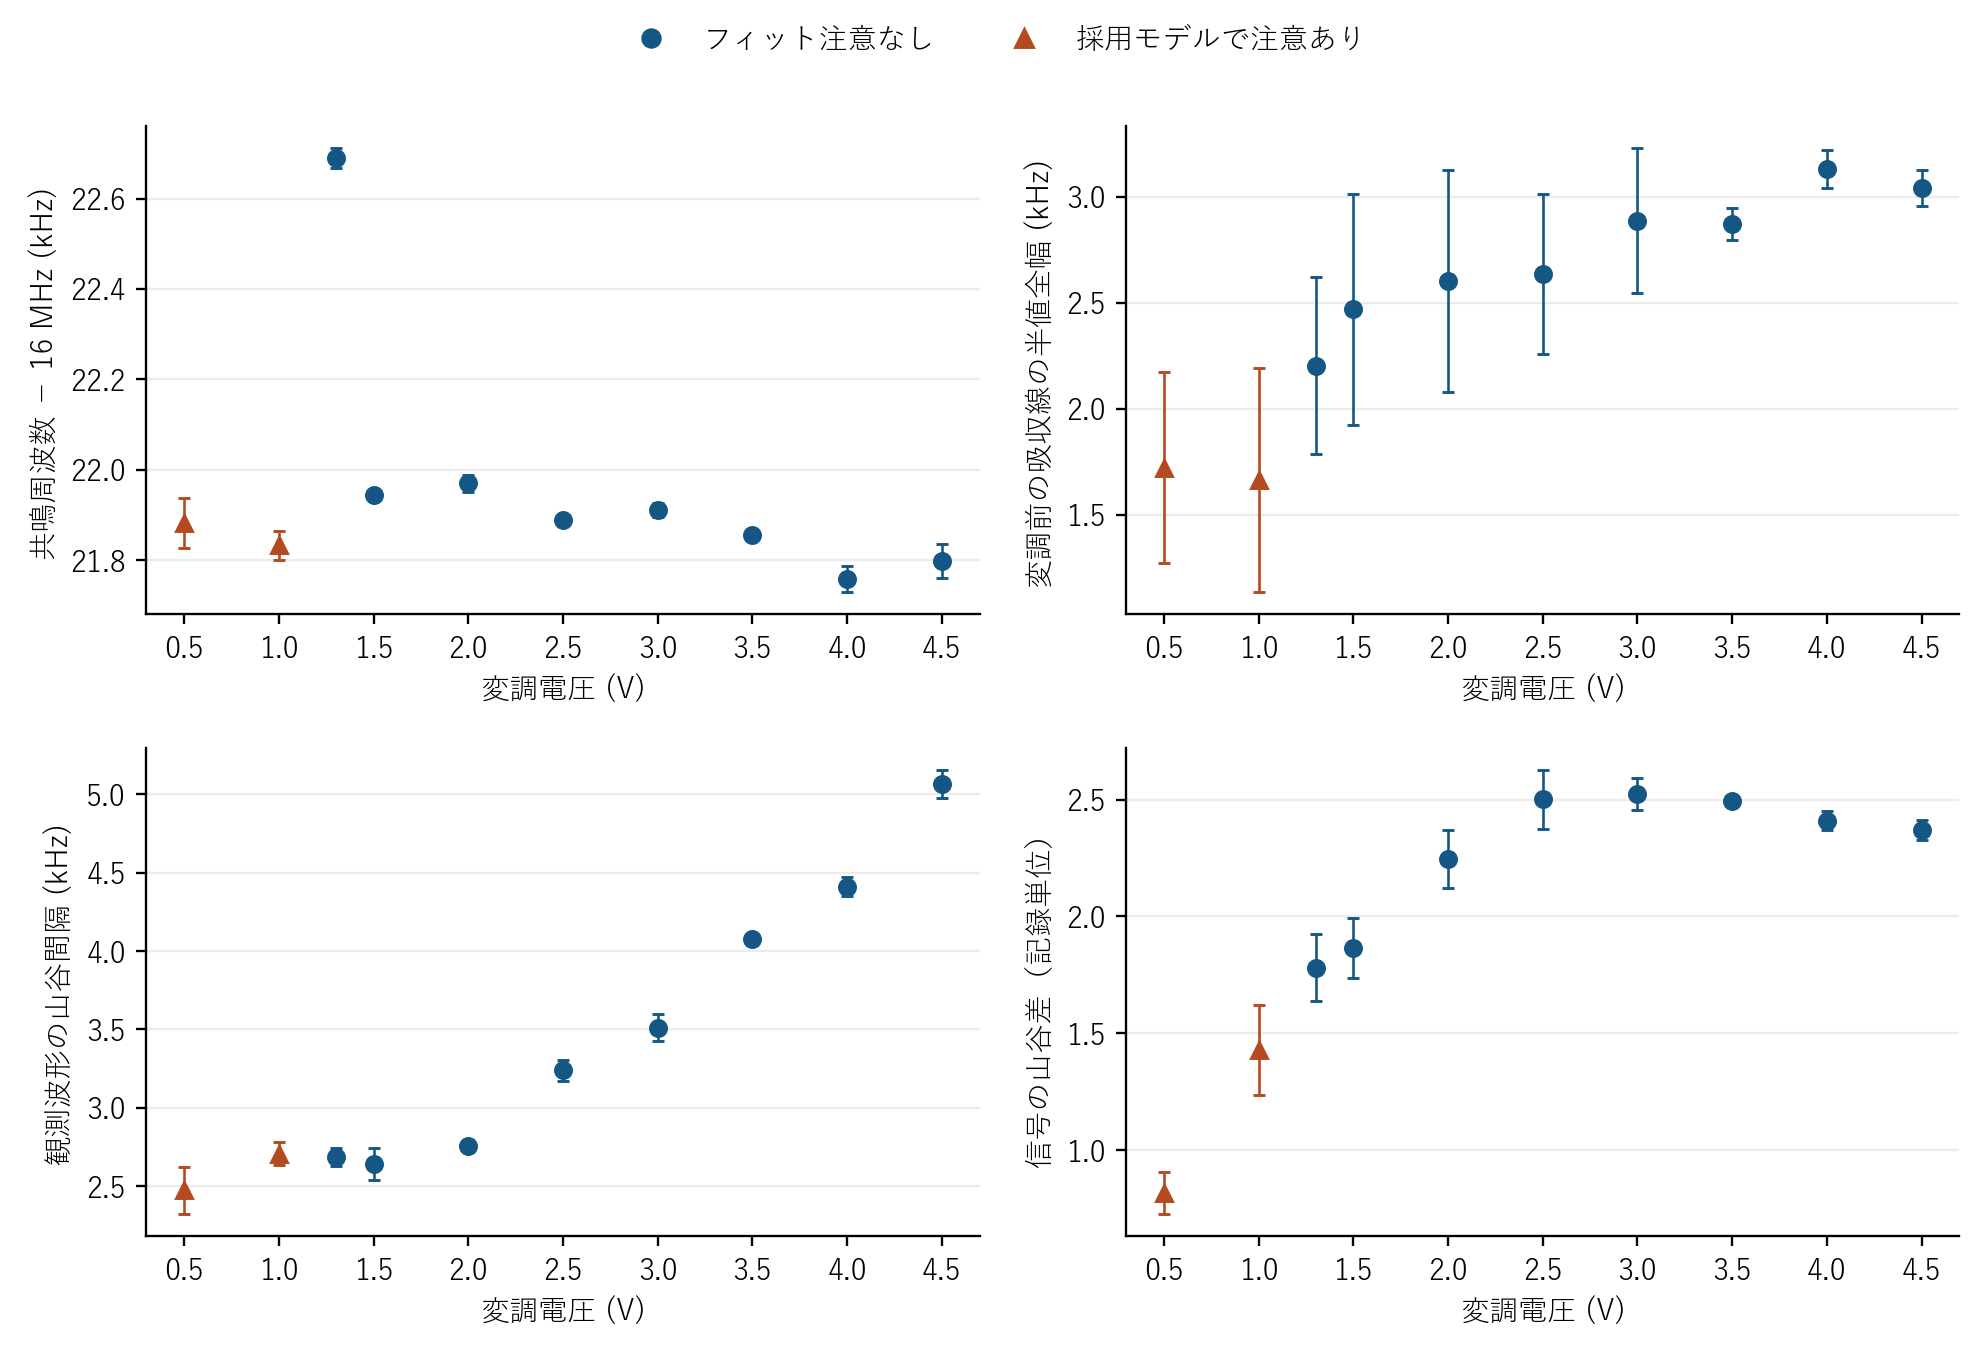
\includegraphics[width=.95\linewidth]{fig4.png}
  \caption{変調周波数280 Hzにおける電圧依存性。有限変調Voigt型による各量の推定値と標準不確かさを示す。三角印は有限変調Voigt型のフィットに注意が付いた条件。}\label{fig:task3-voltage}
\end{figure}

図\ref{fig:task3-models}に\SI{4.5}{\volt}の代表波形を示す。予測RMSは微分ローレンツ型で0.314、微分Voigt型で0.161、有限変調Voigt型で0.099となった。
有限変調ローレンツ型でも0.102まで下がり、この条件では変調を計算に含める効果が大きかった。

\begin{figure}[htbp]
  \centering
  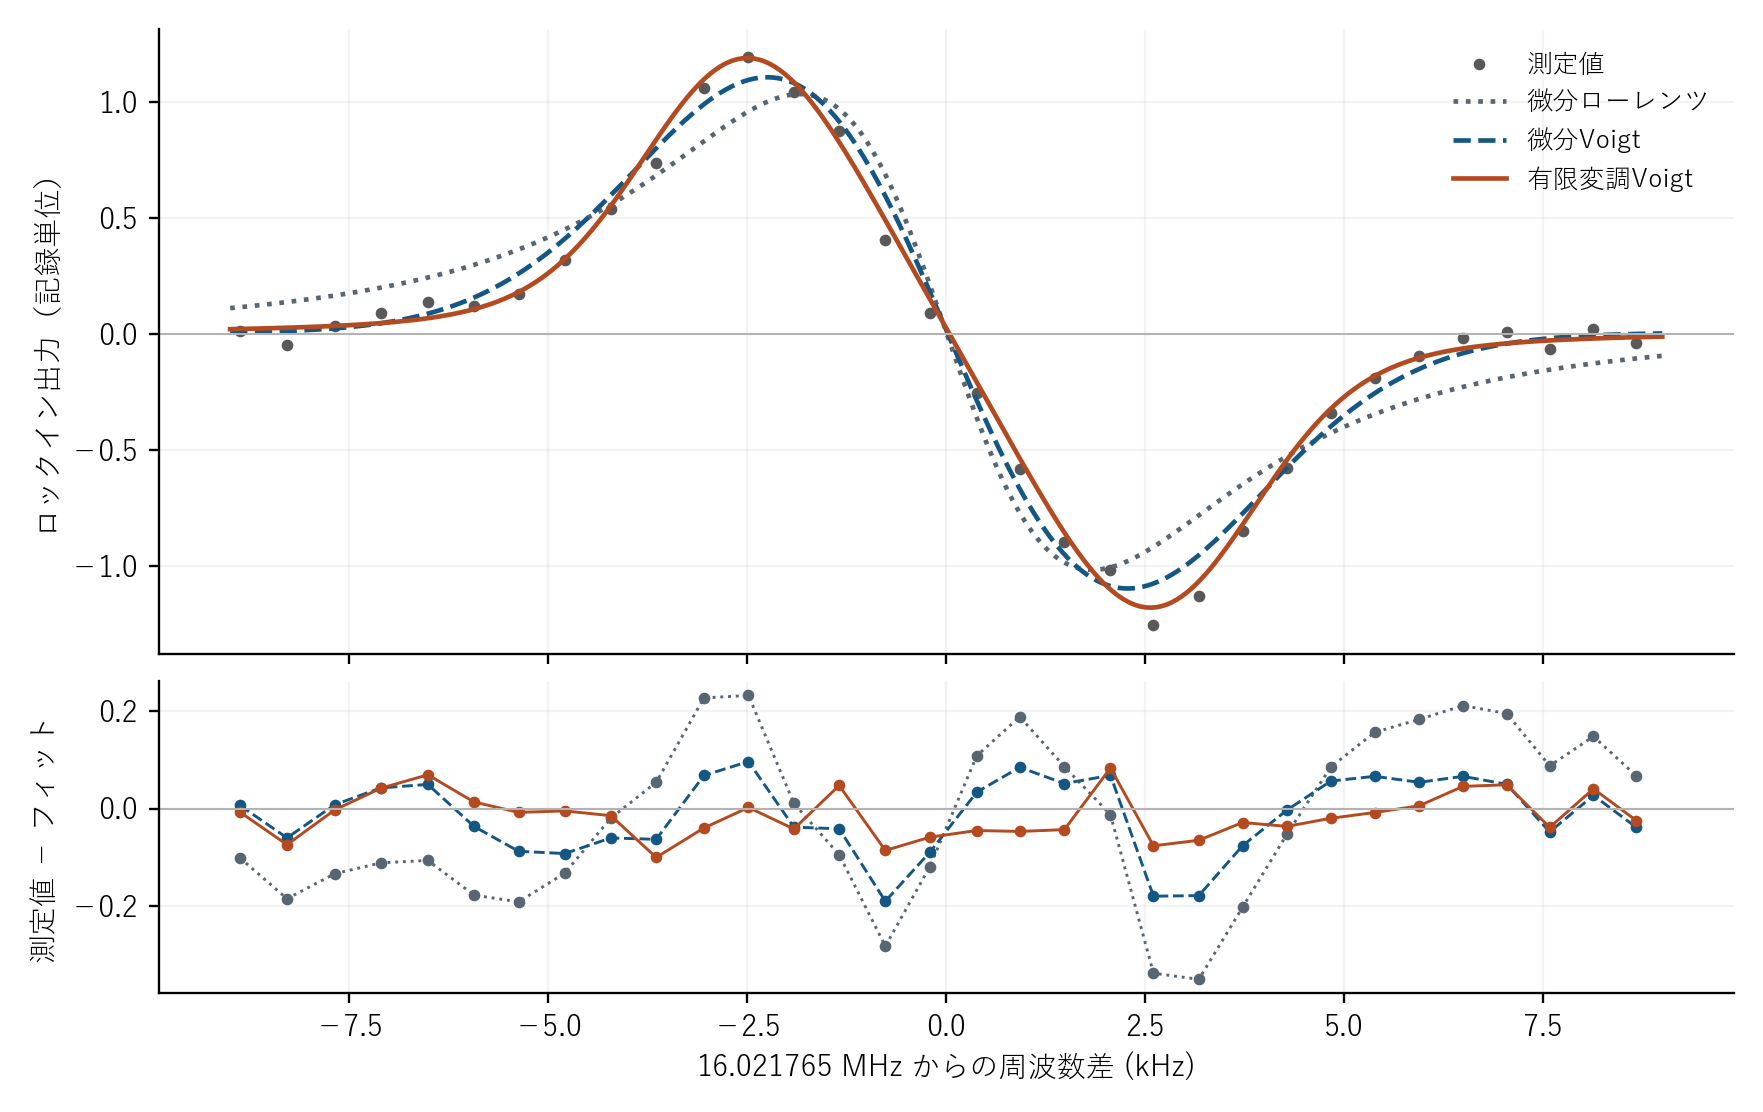
\includegraphics[width=.87\linewidth]{fig6.png}
  \caption{4.5 V・280 Hzにおける測定値、三つのフィット曲線と残差。各モデルを全測定点に当てはめ、共鳴近傍を拡大表示した。}\label{fig:task3-models}
\end{figure}

\paragraph{追加測定：変調周波数依存性}
電圧表示を\SI{1.3}{\volt}に固定した20条件のうち、20 Hzと60 Hzはそれぞれ基準解析時の弱信号・短い背景範囲、周期的な背景を理由に参考条件とし、残る18条件を定量比較した。
40 Hzと400 Hzにおける観測基本波の山谷間隔はそれぞれ\SI{9.08}{\kilo\hertz}、\SI{2.78}{\kilo\hertz}であった。
120、180、240 Hzでは共鳴から離れた部分にも構造が見られ、特に120 Hzの吸収線幅は\SI{1.91(73)}{\kilo\hertz}と推定のばらつきが大きい。

\begin{figure}[htbp]
  \centering
  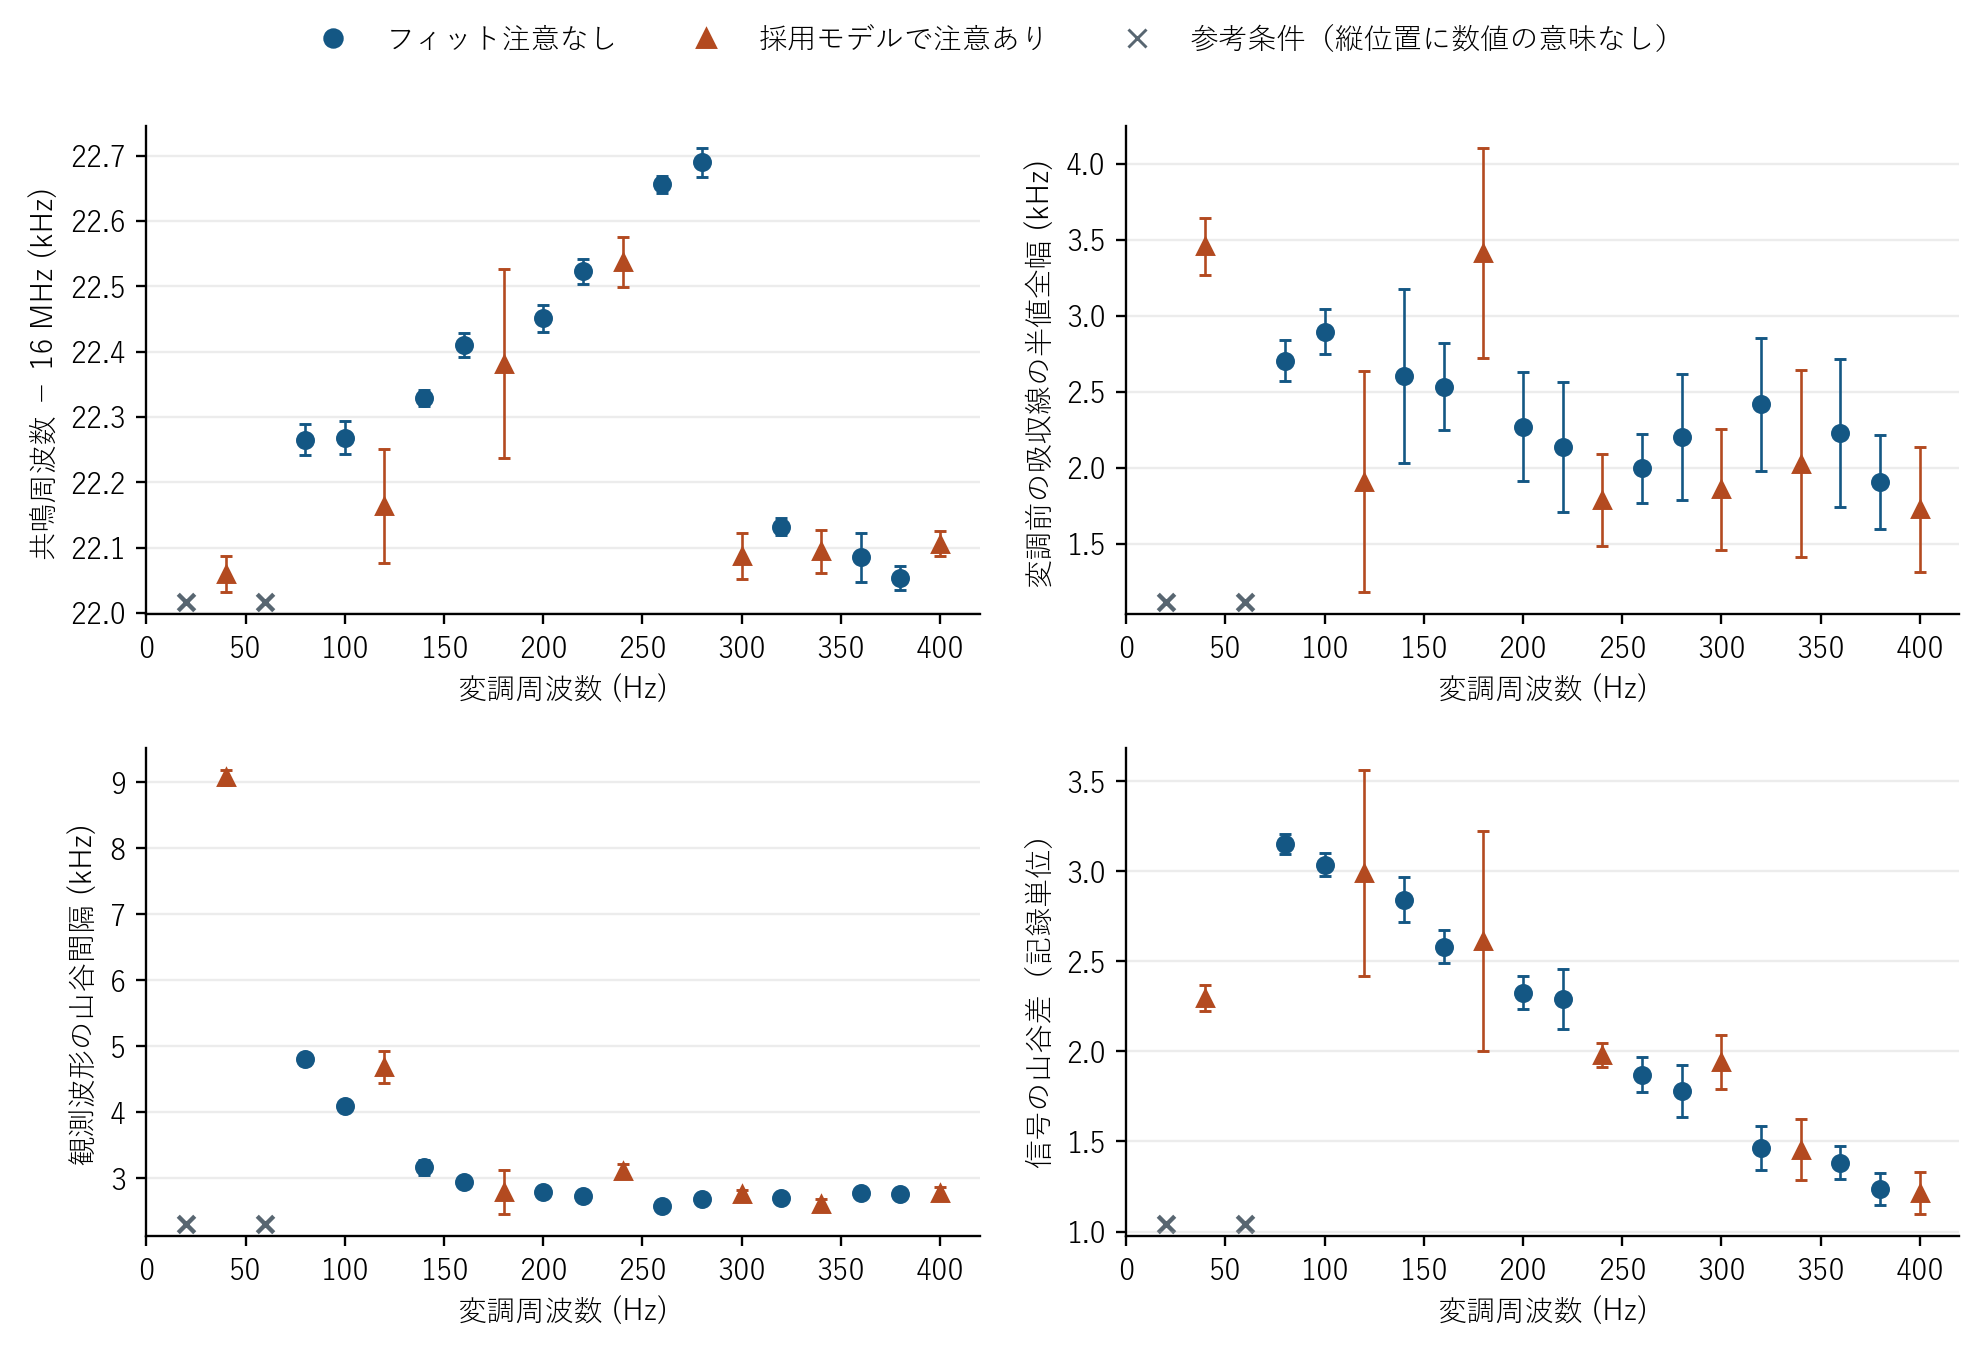
\includegraphics[width=.95\linewidth]{fig5.png}
  \caption{電圧表示1.3 Vにおける周波数依存性。20、60 Hzの灰色の印は横軸上の参考条件の位置を示し、その縦位置に測定値の意味はない。誤差棒は標準不確かさ、三角印は有限変調Voigt型のフィットに注意が付いた条件。}\label{fig:task3-frequency}
\end{figure}

\subsection{残差と推定の信頼性}
課題2・3の注意判定には、それぞれの採用モデルによる全測定点の残差を用いた。
隣り合う残差の相関係数の絶対値が0.30を超えたのは、課題2で78座標中22座標、課題3で27条件中4条件（1.3 Vの120、180、240、300 Hz）であった。
課題3の4.5 V・280 Hzではこの相関係数は0.064であった。
弱信号の目安は、背景を引いたフィット波形の山谷差の半分を残差標準偏差（自由度補正あり）で割った値が5未満の場合とした。
中心から近い掃引端までの距離が吸収線の半値全幅に満たない場合、線幅の相対標準不確かさが25\%以上の場合、形状パラメータが下限付近に達した場合にも注意を付けた。
定量採用点でも10月28日の$(2.5,6.0)$は弱信号で、微分Voigt型による吸収線幅は\SI{7.57(146)}{\kilo\hertz}となった。
課題3では、二系列に共通の1.3 V・280 Hzを1件と数えた27条件すべてで、微分Voigt型は微分ローレンツ型より予測RMSが小さかった（減少率の中央値33.1\%）。
有限変調Voigt型と微分Voigt型を比べた予測RMSの減少率の中央値は0.8\%で、変調の扱いによる違いは条件ごとに異なる。

\section{考察}
\label{sec:discussion}

\subsection{水素核の共鳴条件と測定結果}
配布テキストに示された磁束密度の目安\SI{0.38}{\tesla}を式\eqref{eq:resonance}に代入すると、
水素核の共鳴周波数は約\SI{16.18}{\mega\hertz}となる。
課題1で得た\SI{16.010623}{\mega\hertz}はこれより約\SI{0.17}{\mega\hertz}低く、
共鳴条件から逆算した磁束密度は約\SI{0.376}{\tesla}である。
したがって、試料から観測された共鳴は、装置の磁場の目安から予想した周波数帯にあった。
磁束密度の目安は試料位置で独立に測った値ではなく、課題1の試料座標も不明である。
周波数差を解釈するには、その位置での磁場の実測値と周波数計の校正情報が必要となる。

共鳴付近ではVoigtモデルのほうが微分ローレンツ型より残差が小さかったが、波形だけから広がりの内訳を決めるのは難しい。
例えば変調片振幅を\SI{1.0}{\kilo\hertz}に固定してフィットし直すと、
ガウス分布の幅は\SI{1.03}{\kilo\hertz}から\SI{0.87}{\kilo\hertz}に変化した一方、
全範囲での残差の二乗平均平方根は0.050689から0.050696への変化にとどまった。
変調片振幅と試料内の周波数分布の幅が互いに補い合うためである。
一方、フィット範囲を共鳴付近の前後5、10、15、\SI{30}{\kilo\hertz}と変えた比較で、共鳴中心の変動は約\SI{0.87}{\hertz}であった。
今回のモデルとデータでは、共鳴中心は幅の内訳より安定して求まった。
共鳴周波数の標準不確かさ約\SI{21}{\hertz}は残差モデルのもとでの見積もりであり、装置全体の測定精度を評価するには校正や掃引条件の確認も必要である。

\subsection{磁場の一様性とNMR用磁石に求められる条件}
11月10日の$x=4.5$の測定では、$z$が大きくなるにつれて半値全幅が減少し、信号強度は増加した。
試料には有限の大きさがあるため、試料内で静磁場が変化すると、核スピンの共鳴周波数にも分布が生じる。
この分布は吸収線を広げ、信号の山谷差にも影響する。NMR測定に用いる磁石には、試料全体での磁場の一様性と測定中の安定性が求められる。
今回の線幅や強度には、磁場変調や検出系の応答の影響も含まれるため、線幅だけから試料内の磁場勾配を求めることは難しい。

同一座標で観測された日付間の平均差\SI{9.675}{\kilo\hertz}を磁束密度に換算すると、
約\SI{0.227}{\milli\tesla}に相当する。
この差があるため、測定日が切り替わる境界の段差を、磁場の空間的な変化としてそのまま解釈することはできない。
ロックインアンプの設定は同じであった。磁場の経時変化や試料位置の再現性はこの比較だけでは切り分けられず、
4点の差を他の座標や11月4日の測定に適用できるかも未確認である。

\subsection{磁場変調振幅の影響と横緩和時間}
微小変調では、他の測定条件が一定であればロックイン出力の基本波成分は変調磁場振幅にほぼ比例する。
電圧を低い側から上げると山谷差が増えた一方、高い側では観測波形の山谷間隔が引き続き増え、山谷差は緩やかに減少した。
変調による共鳴周波数の振れが大きくなると、吸収線の局所的な傾きで信号を近似できる範囲を外れ、波形の山と谷の位置や高さが変わる。
高電圧で有限変調を入れたモデルの残差が小さくなったことは、見かけの線幅の増加に有限変調が関わるという解釈と整合する。

$T_2$を線幅から求める式$\Delta f_{\mathrm{FWHM}}=1/(\pi T_2)$は、均一磁場かつ弱い高周波励起でのローレンツ吸収線に対応する。
一方、波形への適合度が近い解でも、変調幅、試料内の共鳴周波数分布の幅、ローレンツ幅の内訳は異なり得る。
例えば\SI{0.5}{\volt}の測定では、変調片振幅をゼロに固定した解と自由に推定した解の残差平方和の差は約1.3\%であったが、
ローレンツ半値半幅$\Gamma$はそれぞれ約\SI{0.21}{\kilo\hertz}と\SI{0.57}{\kilo\hertz}となった。
これらを形式的に$T_2=1/(2\pi\Gamma)$に換算すると、約\SI{0.76}{\milli\second}と\SI{0.28}{\milli\second}となる。
この差は、同程度に波形を説明できても、推定される緩和時間が大きく変わることを示している。

したがって、今回の測定からは変調条件による見かけの線幅の変化を確認できたが、物質固有の$T_2$を一意に決定するには至らなかった。
変調電圧から試料位置での磁場振幅への換算も未確認であり、定量評価には、変調磁場の校正、試料内の磁場不均一による広がり、および検出系の時間応答の評価が必要である。

追加測定の周波数系列では、駆動電圧の表示値を固定しても、コイルの電流応答によって変調磁場振幅が変わり得る。
ロックイン検出と掃引の時間応答も波形に影響し得るため、周波数による線幅の変化を試料の緩和だけに帰属させるには、変調磁場と検出条件の確認が必要である。

\subsection{モデルの妥当性と不確かさ}
微分Voigt型を用いると、課題2の大半の位置と課題3の定量採用全条件で、微分ローレンツ型より未使用区間をよく予測できた。
課題2の共鳴中心は線形を変えても比較的安定で、線幅の方がモデル選択の影響を受けた。課題3の高電圧側では観測基本波の幅が大きくなるため、有限変調を含めた解析から変調前の吸収線幅と観測波形の幅を区別する必要がある。
いずれの不確かさも仮定した平均波形のもとでの推定であり、左右非対称性や周期的な背景の起源までは決定できない。

\subsection{測定の限界と改善案}
位置依存性を測定日間で比較するには、複数の共通座標を各日の測定の前後で測り、日付間の差と測定中の変化を調べる。
また、同じ条件で掃引方向や待ち時間を変えれば、検出系の応答遅れが共鳴中心や波形に及ぼす影響を評価できる。
線幅から$T_2$を評価するには、試料位置での変調磁場振幅を校正し、小さな変調振幅で波形を測定することに加え、試料内の磁場分布による広がりを評価する必要がある。
ゼロ変調への外挿を行う場合にも、外挿後の線幅に含まれる磁場不均一や検出系の応答の寄与を検討する必要がある。

\clearpage
\section{NMRの応用例}
\label{sec:applications}

磁気共鳴画像法（MRI）では、体内の水や脂肪に含まれる水素核を静磁場中で高周波パルスによって励起する。
励起後に歳差運動する横磁化が受信コイルに誘起する電圧を、時間信号として測定する\cite{nibib_mri,mansfield_mri}。
縦磁化の回復を特徴づける$T_1$は次の励起で得られる信号の大きさに関わり、横磁化の減衰を特徴づける$T_2$はスピンエコーの信号強度に関わる。
パルスの繰り返し間隔やエコーを観測する時刻を選ぶことで、組織間の緩和の違いを画像の明暗に反映できる\cite{nibib_mri,mansfield_mri}。

共鳴周波数が局所の磁束密度に比例するため、傾斜磁場を加えると、横磁化が歳差運動する周波数や位相に位置の情報が入る。
複数の傾斜磁場の条件で測った信号から空間分布を再構成する\cite{mansfield_mri}。
課題2では、既知の位置に試料を移動し、その共鳴周波数から磁束密度を求めた。
MRIでは同じ共鳴条件を利用し、既知の傾斜磁場を加えて測定信号に位置の情報を持たせる。

% ===== 参考文献 =====
% 本文中では \cite{manual} のように引用する。
% 著者、資料名、発行年、該当ページ等を確認して記入する。
% Web資料はURLに加えて閲覧日を記す。
\begin{thebibliography}{99}
  \bibitem{manual}
  物理学実験テキスト「核磁気共鳴」，配布資料，pp.~1--10，18--24，26．
  % ローカル資料：../10核磁気共鳴.pdf。著者・年度は資料の正式情報を確認して追記する。

  \bibitem{efron_bootstrap}
  B. Efron and R. J. Tibshirani, \textit{An Introduction to the Bootstrap},
  Chapman \& Hall (1993), Chap.~6, especially Sec.~6.5.
  \href{https://doi.org/10.1201/9780429246593}{doi:10.1201/9780429246593}.

  \bibitem{smeekes_wilms_bwb}
  S. Smeekes and I. Wilms, \textit{bootUR: An R Package for Bootstrap Unit Root Tests},
  Journal of Statistical Software \textbf{106}(12) (2023), Sec.~3.4.
  \href{https://doi.org/10.18637/jss.v106.i12}{doi:10.18637/jss.v106.i12}.

  \bibitem{mackinnon_hc1}
  J. G. MacKinnon, \textit{Thirty Years of Heteroskedasticity-Robust Inference},
  Queen's Economics Department Working Paper No.~1268 (2011, revised 2014),
  \href{https://qed.econ.queensu.ca/working_papers/papers/qed_wp_1268.pdf}{variants w1u1 and w1u2}.

  \bibitem{nibib_mri}
  National Institute of Biomedical Imaging and Bioengineering, ``Magnetic Resonance Imaging (MRI),''
  \href{https://www.nibib.nih.gov/science-education/science-topics/magnetic-resonance-imaging-mri}{NIBIB Science Topics}（2026年11月15日閲覧）．

  \bibitem{mansfield_mri}
  P. Mansfield, ``Snap-Shot MRI,'' Nobel Lecture, 8 December 2003, pp.~266--270,
  \href{https://www.nobelprize.org/uploads/2018/06/mansfield-lecture.pdf}{NobelPrize.org}（2026年11月15日閲覧）．
\end{thebibliography}

\end{document}
